%%%%%%%%%%%%%%%%%%%%%%%%%%%%%%%%%%%%%%%
% Cathal Harte CV1 based on:
%
% Wenneker Resume/CV
% LaTeX Template
% Version 1.1 (19/6/2016)
%
% This template has been downloaded from:
% http://www.LaTeXTemplates.com
%
% Original author:
% Frits Wenneker (http://www.howtotex.com) with extensive modifications by 
% Vel (vel@LaTeXTemplates.com)
%
% License:
% CC BY-NC-SA 3.0 (http://creativecommons.org/licenses/by-nc-sa/3.0/
%
%%%%%%%%%%%%%%%%%%%%%%%%%%%%%%%%%%%%%%

%----------------------------------------------------------------------------------------
%	PACKAGES AND OTHER DOCUMENT CONFIGURATIONS
%----------------------------------------------------------------------------------------

\documentclass[a4paper,12pt]{memoir} % Font and paper size

%%%%%%%%%%%%%%%%%%%%%%%%%%%%%%%%%%%%%%%%%
% Wenneker Resume/CV
% Structure Specification File
% Version 1.1 (19/6/2016)
%
% This file has been downloaded from:
% http://www.LaTeXTemplates.com
%
% Original author:
% Frits Wenneker (http://www.howtotex.com) with extensive modifications by 
% Vel (vel@latextemplates.com)
%
% License:
% CC BY-NC-SA 3.0 (http://creativecommons.org/licenses/by-nc-sa/3.0/)
%
%%%%%%%%%%%%%%%%%%%%%%%%%%%%%%%%%%%%%%%%%

%----------------------------------------------------------------------------------------
%	PACKAGES AND OTHER DOCUMENT CONFIGURATIONS
%----------------------------------------------------------------------------------------

\usepackage{XCharter} % Use the Bitstream Charter font
\usepackage[utf8]{inputenc} % Required for inputting international characters
\usepackage[T1]{fontenc} % Output font encoding for international characters

\usepackage[top=1cm,left=1cm,right=1cm,bottom=1cm]{geometry} % Modify margins

\usepackage{graphicx} % Required for figures

\usepackage{flowfram} % Required for the multi-column layout

\usepackage{url} % URLs

\usepackage[usenames,dvipsnames]{xcolor} % Required for custom colours

\usepackage{tikz} % Required for the horizontal rule

\usepackage{enumitem} % Required for modifying lists
\setlist{noitemsep,nolistsep} % Remove spacing within and around lists

\setlength{\columnsep}{\baselineskip} % Set the spacing between columns

% Define the left frame (sidebar)
\newflowframe{0.2\textwidth}{\textheight}{0pt}{0pt}[left]
\newlength{\LeftMainSep}
\setlength{\LeftMainSep}{0.2\textwidth}
\addtolength{\LeftMainSep}{1\columnsep}
 
% Small static frame for the vertical line
\newstaticframe{1.5pt}{\textheight}{\LeftMainSep}{0pt}
 
% Content of the static frame with the vertical line
\begin{staticcontents}{1}
\hfill
\tikz{\draw[loosely dotted,color=RoyalBlue,line width=1.5pt,yshift=0](0,0) -- (0,\textheight);}
\hfill\mbox{}
\end{staticcontents}
 
% Define the right frame (main body)
\addtolength{\LeftMainSep}{1.5pt}
\addtolength{\LeftMainSep}{1\columnsep}
\newflowframe{0.7\textwidth}{\textheight}{\LeftMainSep}{0pt}[main01]

\pagestyle{empty} % Disable all page numbering

\setlength{\parindent}{0pt} % Stop paragraph indentation

%----------------------------------------------------------------------------------------
%	NEW COMMANDS
%----------------------------------------------------------------------------------------

\newcommand{\userinformation}[1]{\renewcommand{\userinformation}{#1}} % Define a new command for the CV user's information that goes into the left column

\newcommand{\cvheading}[1]{{\Huge\bfseries\color{RoyalBlue} #1} \par\vspace{.6\baselineskip}} % New command for the CV heading
\newcommand{\cvsubheading}[1]{{\Large\bfseries #1} \bigbreak} % New command for the CV subheading

\newcommand{\Sep}{\vspace{1em}} % New command for the spacing between headings
\newcommand{\SmallSep}{\vspace{0.5em}} % New command for the spacing within headings

\newcommand{\aboutme}[2]{ % New command for the about me section
\textbf{\color{RoyalBlue} #1}~~#2\par\Sep
}
	
\newcommand{\CVSection}[1]{ % New command for the headings within sections
{\Large\textbf{#1}}\par
\SmallSep % Used for spacing
}

\newcommand{\CVItem}[2]{ % New command for the item descriptions
\textbf{\color{RoyalBlue} #1}\par
#2
\SmallSep % Used for spacing
}

\newcommand{\bluebullet}{\textcolor{RoyalBlue}{$\circ$}~~} % New command for the blue bullets
 % Include the file specifying document layout and packages

%----------------------------------------------------------------------------------------
%	NAME AND CONTACT INFORMATION 
%----------------------------------------------------------------------------------------

\userinformation{ % Set the content that goes into the sidebar of each page
\begin{flushright}
% Comment out this figure block if you don't want a photo
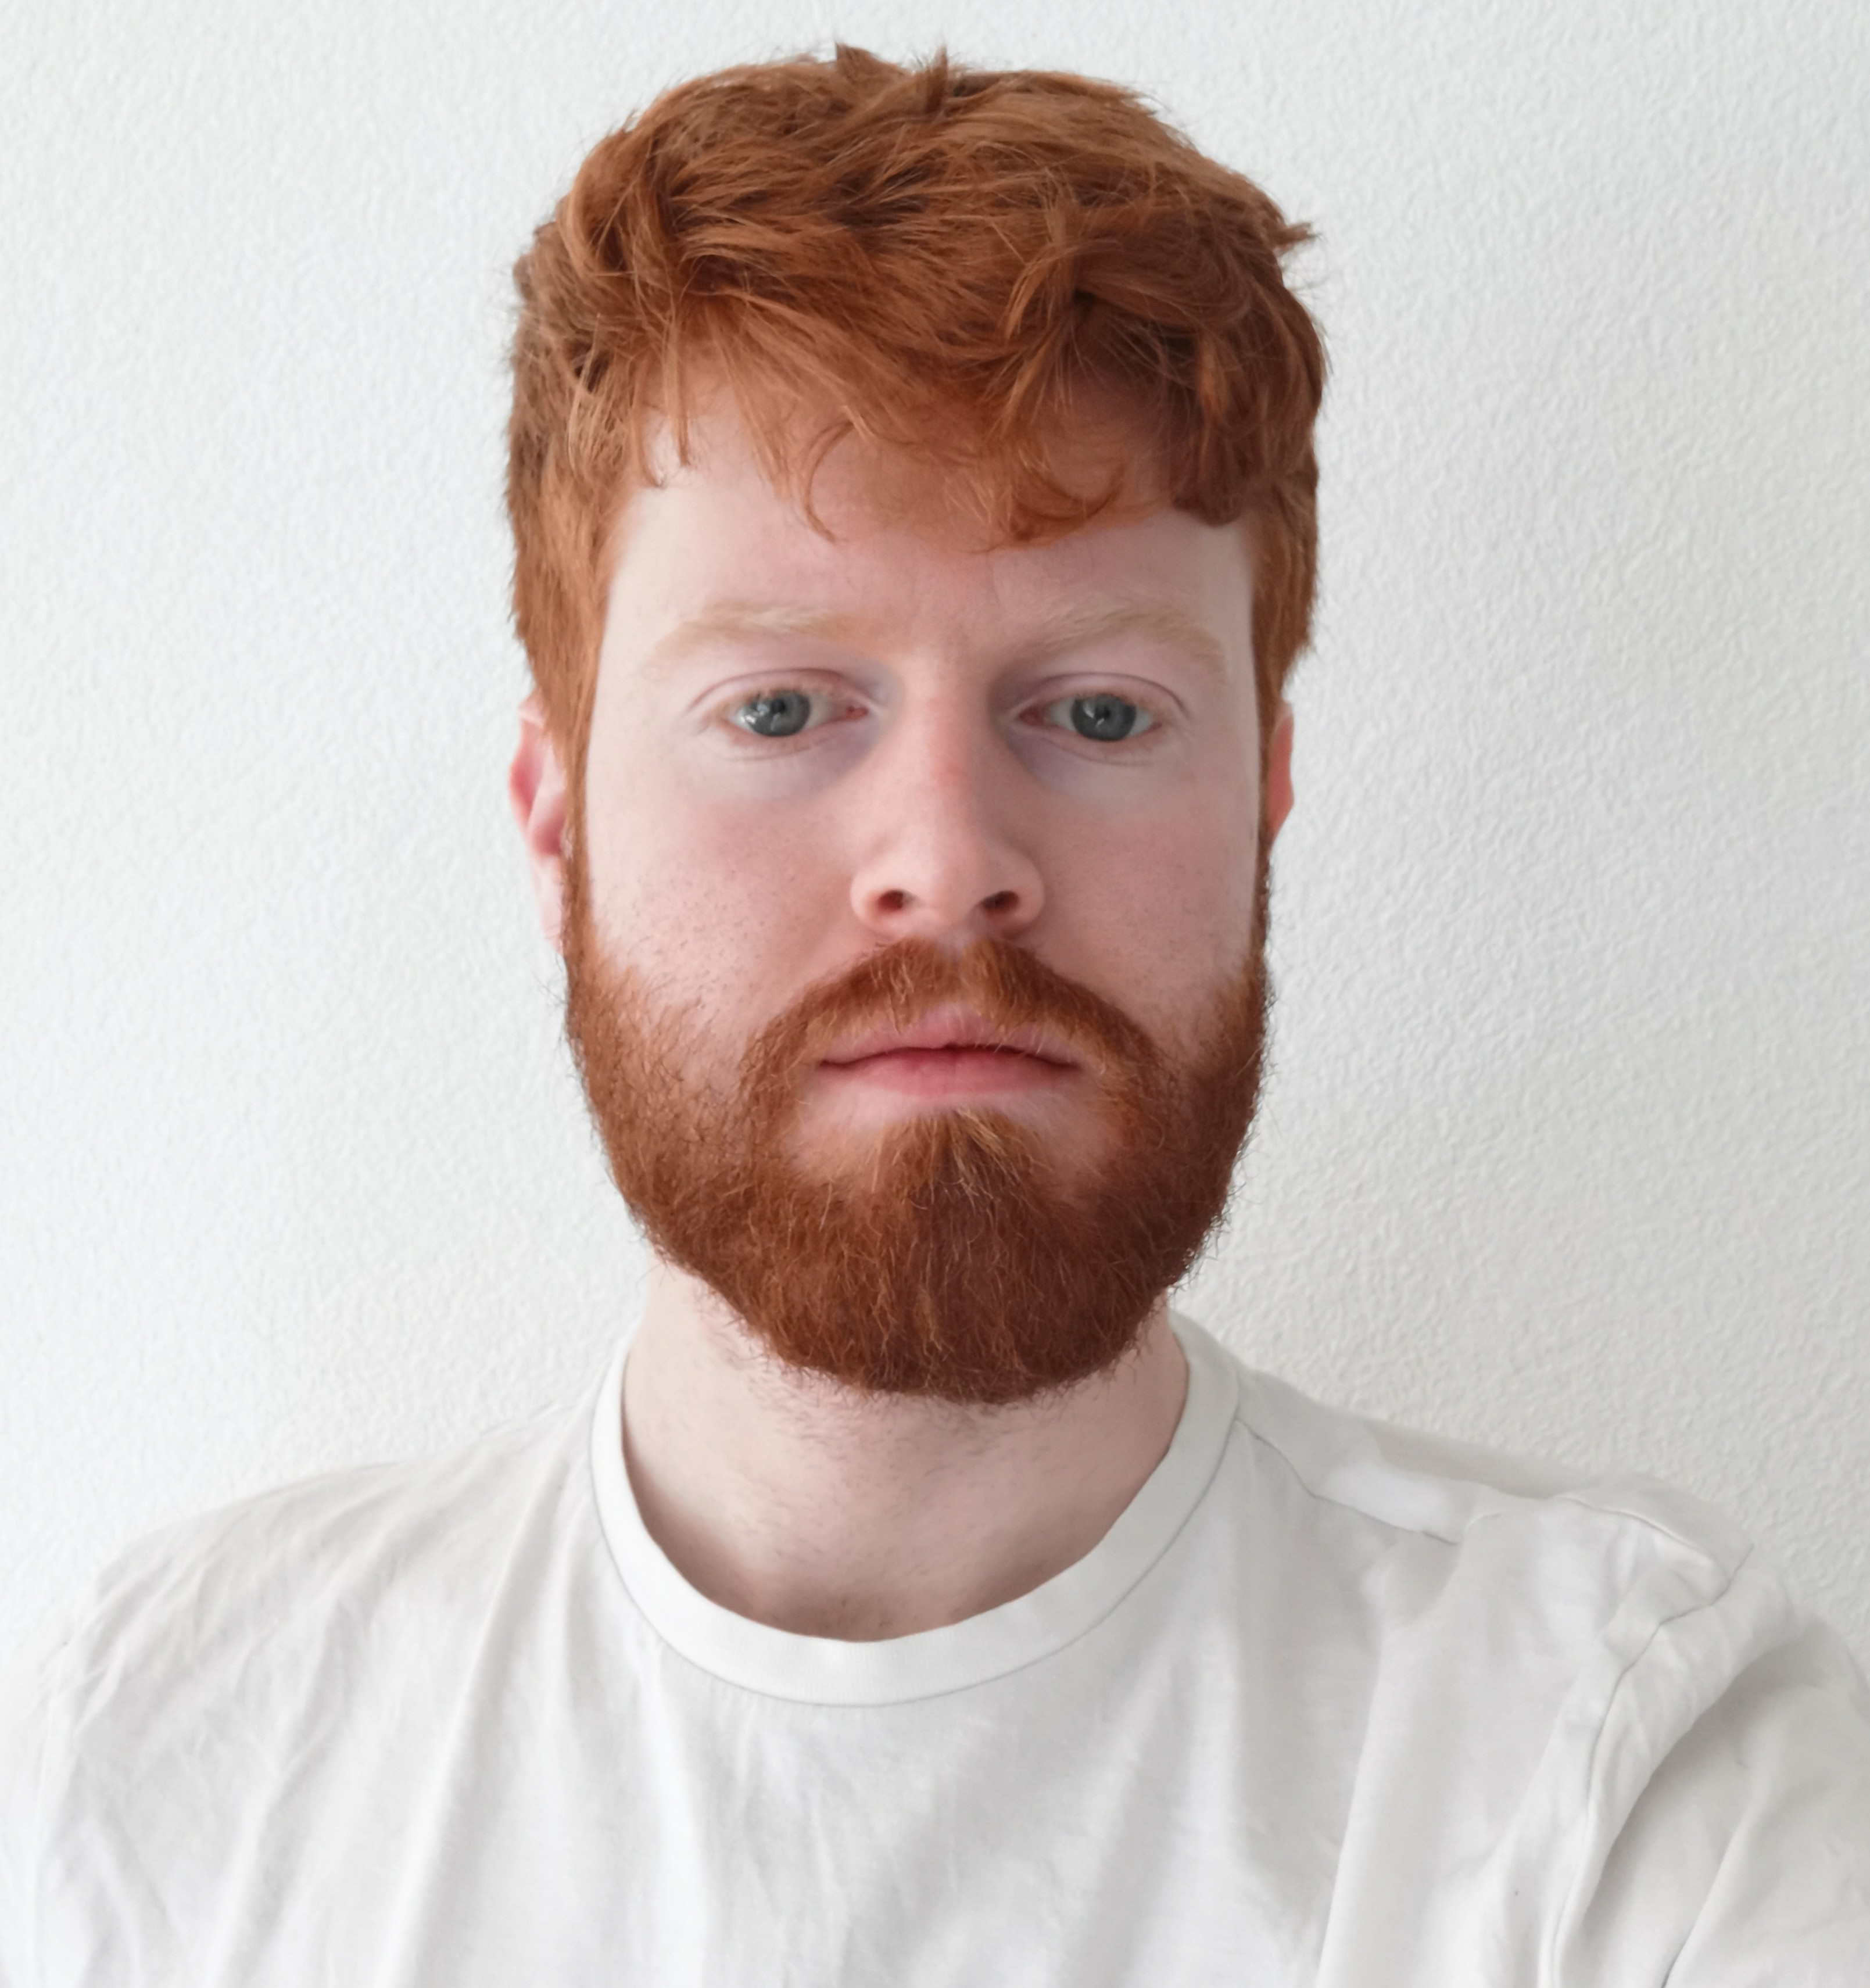
\includegraphics[width=0.6\columnwidth]{mugshot.jpg}\\[\baselineskip] % Your photo
\small % Smaller font size
Cathal Harte \\ % Your name
\url{cathal.harte@protonmail.com} \\ % Your email address
\url{https://github.com/CathalHarte/} \\ % Your URL
+41 76 480 7891 \\ % Your phone number
\Sep % Some whitespace
\textbf{Address} \\
Rue des Alpes 65 \\ % Address 1
1023 Crissier \\ % Address 2
Vaud \\ % Address 3
\vfill % Whitespace under this block to push it up under the photo
\end{flushright}
}

%----------------------------------------------------------------------------------------

\begin{document}

\userinformation % Print your information in the left column

\framebreak % End of the first column

%----------------------------------------------------------------------------------------
%	HEADING
%----------------------------------------------------------------------------------------

\cvheading{Cathal Harte} % Large heading - your name

\cvsubheading{Software Engineer} % Subheading - your occupation/specialization

%----------------------------------------------------------------------------------------
%	ABOUT ME
%----------------------------------------------------------------------------------------

\aboutme{About Me}{What can I say. Just your average engineer, possessing all the vital characteristics as determined by Larry Wall. Add a touch of spite and thrift as identified by hackaday, and you've got yourself a real contender.}

%----------------------------------------------------------------------------------------
%	EDUCATION
%----------------------------------------------------------------------------------------

\CVSection{Education}

%------------------------------------------------

\CVItem{2016 - 2018, University College Dublin, Ireland}{ME Electronic and Computer Engineering}

\begin{itemize}
	\item Graduated with 2:1 honours, GPA 3.5
	\item Notable results:
	\begin{itemize}
		\item Optimization techniques (A+)
		\item Software Engineering (A)
	\end{itemize}

\end{itemize}


%------------------------------------------------

\CVItem{2013 - 2016, University College Dublin, Ireland}{Bachelor of Science Electronic Engineering}
\begin{itemize}
	\item Completed Bachelor of Science with 2:1 honours degree, GPA 3.62
	\item Notable results: 
	\begin{itemize}
		\item Biomedical Signals and Images(A) 
		\item Digital System Design (A-) 
		\item Computer Science for Engineers II (A) 	
		\item Multivariable Calculus for Engineers (A+) 
		\item Introduction to Artificial Intelligence (A)
	\end{itemize}
\end{itemize}

%------------------------------------------------

\Sep % Extra whitespace after the end of a major section

%----------------------------------------------------------------------------------------
%	EXPERIENCE
%----------------------------------------------------------------------------------------

\CVSection{Experience}

%------------------------------------------------

\CVItem{July 2018 - February 2020, \textit{Systems Engineer}, Rapt Touch SA}{
Achievements:
\begin{itemize}
	\item Developed sensor firmware for the "Spencer" optical touch screen project
	\begin{itemize}
		\item Rapid prototyping leading to a design win with Chinese touch screen market leader.
		\item Production firmware development
		\item Travelled to Shenzhen to aid in mass production "bring up" huh?
	\end{itemize}
\end{itemize}
}
\CVItem{January 2017 - September 2017, \textit{Intern Engineer}, Rapt Touch}{
Achievements:
\begin{itemize}
	\item Developed visualisation tools for Rapt’s touch calculation software.
	\item Developed a regression testing framework utilising the Google Cloud Platform.
	\item Transient analysis and simulation of photodetectors for use in fast pulsed detection systems.
\end{itemize}
}

%------------------------------------------------

\Sep % Extra whitespace after the end of a major section

%------------------------------------------------

\Sep % Extra whitespace after the end of a major section

%----------------------------------------------------------------------------------------
%	NEW PAGE DELIMITER
%	Place this block wherever you would like the content of your CV to go onto the next page
%----------------------------------------------------------------------------------------

\clearpage % Start a new page

\userinformation % Print your information in the left column

\framebreak % End of the first column

%----------------------------------------------------------------------------------------
%	SKILLS
%----------------------------------------------------------------------------------------

\CVSection{Software Development Skills}

%------------------------------------------------

\CVItem{Programming Languages}
{\begin{tabular}{p{0.2\textwidth} p{0.2\textwidth} p{0.2\textwidth}}
\bluebullet C &  \bluebullet C++ & \bluebullet CMake\\
\bluebullet Bash &  \bluebullet Python3 & \bluebullet GoLang\\
\bluebullet Matlab &  \bluebullet Groovy & \bluebullet Java\\
\end{tabular}}

%------------------------------------------------

\CVItem{Architectures}
{\begin{tabular}{p{0.2\textwidth} p{0.2\textwidth} p{0.2\textwidth}}
\bluebullet Cortex-M &  \bluebullet Linux & \bluebullet Android\\
\end{tabular}}

\CVItem{Development Tools}
{\begin{itemize}
	\item JTAG debugging with OpenOCD
	\item Visual Studio Code
	\item Keil - $\mu$Vision IDE and compiler
	\item STM CubeMX code generator
	\item Eclipse IDE
	\item Saleae Logic Analyzer
\end{itemize}
}

\CVItem{Development Techniques}
{\begin{itemize}
	\item Test Driven Development
	\item Modular Design and unit testing
	\item Eric Meijer's One Hacker Way\\
\end{itemize}}

%------------------------------------------------

\Sep % Extra whitespace after the end of a major section

%----------------------------------------------------------------------------------------
%	INTERESTS
%----------------------------------------------------------------------------------------

\CVSection{Interests}

%------------------------------------------------

\CVItem{Professional}{Open source software, autogenerated C code, cloud computing}

%------------------------------------------------

\CVItem{Personal}{Songwriting, cooking, bouldering, skiing, skateboarding, running}

%------------------------------------------------

\Sep % Extra whitespace after the end of a major section

%----------------------------------------------------------------------------------------

\end{document}
